\chapter{Numerical Experiments}
\label{chap:numerical-experiments}

\section{Primal hard-margin SVM}
\label{sec:numerical-example-svm}

A common problem in machine learning
is binary classification, where we are given a dataset
$D := \{\, (a_i, b_i) \mid i\in\{\, 1,\dots,N \,\} \,\}$
of size $N\in\N$, where each
$a_i\in\R^n$ is called \textit{feature}
and each $b_i\in \{ 0, 1 \}$ is called
\textit{label}. As a specific example, one can think of the problem of
classifying images of pets
as either a cat ("$0$") or dog ("$1$").
The features and labels can be seen as samples from an underlying
probability distribution $\Prob$ on the space $\R^n \times \{0, 1\}$.
Given this dataset, we aim to learn a rule to classify 
new samples $a_{n+1}\in\R^n$ from the distribution of the features
as either $0$ or $1$. Ideally this rule would
choose the class that maximizes $\Prob(a_{n+1}, \cdot)$.
One approach to find such a rule is called \textit{support vector machine} (SVM),
which is an algorithm for constructing a hyperplane that seperates the two
subsets $\{\, a\in \R^n \mid (a, 0) \in D  \,\}$
and $\{\, a\in \R^n \mid (a, 1) \in D  \,\}$.
New samples are then classified based
on which side of the hyperplane they lie in.
Whether or not such a hyperplane even exists depends on the nature
of the dataset.  Nevertheless, we can always write down the problem of finding
such a hyperplane as a convex optimization problem
with affine constraints:
\begin{equation}
    \label{eq:svm-hard-margin}
    \tag{SVM}
    \begin{aligned}
    &\min_{x \in \R^n} \,
        \frac{1}{2} |\!|x|\!|^2 \\
    &\textup{s.\,t.}\quad
    b_i \langle a_i, x \rangle \geq 1 \quad\textnormal{for all $i\in\{ \, 1,\dots,N \, \}$}.
    \end{aligned}
\end{equation}
If a solution to the above problem exists, we say that the dataset is
\textit{linearly seperable}.
This is often not the case, which is why the above problem is usually relaxed to the unconstrained problem
\[
    \min_{x\in\R^n} \frac{1}{2} |\!|x|\!|^2 + C \sum_{i=1}^{N} \max(0, 1 - b_i \langle a_i, x \rangle), 
\]
where $C\in (0, \infty)$. This problem always has a solution, regardless of whether
or not the dataset is actually linearly seperable. However,
the quality of its solution for the classification task is highly
dependent on the choice of $C$ \cite{hastie2004entire}. In particular, if $C$ is too
small, the resulting classifier will perform poorly.

In contrast, our \cref{alg:seqprox-sgd} allows us to bypass this problem because we can directly apply it to
\eqref{eq:svm-hard-margin}.
This problem fits our template problem \eqref{eq:main-problem-copy} by taking
$F_\xi(x) \equiv \frac{1}{2}\norm{x}^2$, $r \equiv 0$,
and
\[
    A(a, b) = -b a^\top,
    \qquad
    b(a, b) = -1,
\]
for $(a, b) \in D$.
\begin{figure}[t]
    \centering
    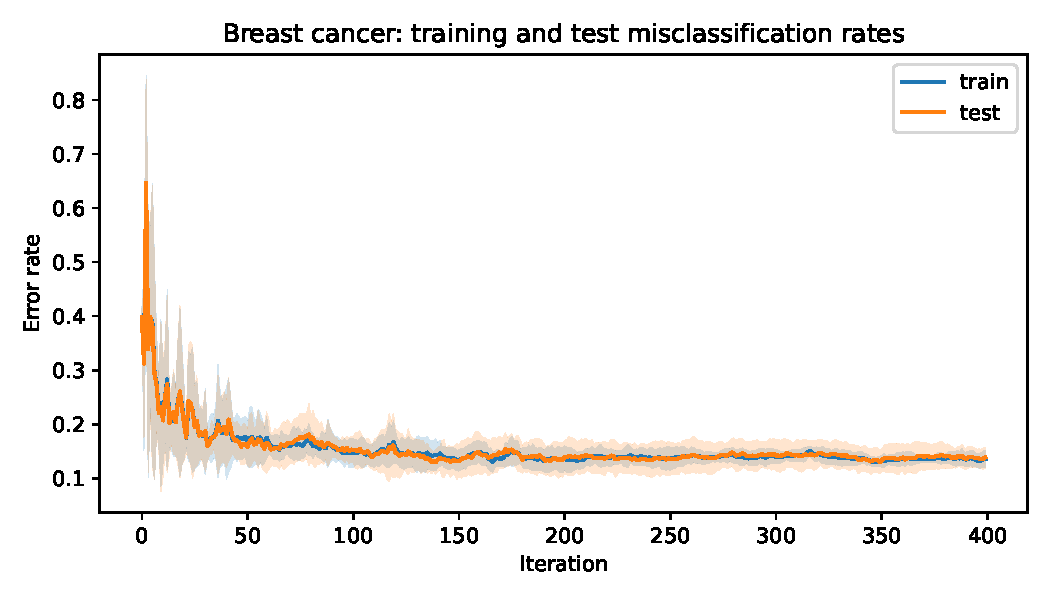
\includegraphics[width=0.75\textwidth]{../code/examples/svm/breast_cancer/sipm_svm_errors.pdf}
    \caption{Breast cancer: training and test misclassification rates over iterations. The shaded regions show $\pm 1$ standard deviations.}
    \label{fig:svm-breast-cancer-errors}
\end{figure}
To test \cref{alg:seqprox-sgd} on real world data, we use the Wisconsin Diagnostic Breast Cancer dataset \cite{breastcancer}
with $n=30$ features and $N=569$ samples.
Features are standardized, and we use a stratified $70/30$ train/test
split\footnote{For background information on machine learning evaluation methods,
see the book \cite{geron2022hands}.}.
To avoid perfect separability, we flip labels independently with probability $0.1$.
As the penalty function sequence $(h_k)_{k\in\N_0}$, we use the Huber-type penalty from (\textcolor{red}{TODO}).
The objective is $1$-strongly convex, so we use the parameter schedule suggested by \cref{cor:convergence-rates-in-expectation}:
\[
    \eta_0 = 2,\qquad
    \eta_k = \frac{2}{k},\qquad
    \gamma_k = \ln(k+1),\qquad
    \delta_0 = 1,\qquad
    \delta_k = \frac{1}{k}, \qquad
    w_k = \eta_k^{-1},
\]
for $k\in\N$.

Since there does not exist a solution to this problem, we will track the
misclassification rates\footnote{The misclassification rate is defined as the percentage of falsely classified examples in a given set.}
of the sequence of iterates $(\bar{x}_k)_{n\in\N}$ generated by \cref{alg:seqprox-sgd}, evaluated
on the training and test sets, respectively.
We repeat the experiment over $10$ independent runs
and report the mean and standard
deviation of the train and test misclassification rates over the sequence of averaged iterates $(\bar{x}_k)_{k\in\N}$.
\Cref{fig:svm-breast-cancer-errors} shows the average training
and test error across iterations with $\pm 1$ standard deviation bands.
After $400$ iterations, the final training error is
$0.1357 \pm 0.0158$ and the final test error is
$0.1386 \pm 0.0192$.

\section{Inventory control}
\label{sec:numerical-example-inventory-control}

This example is adapted from Section~4.8.2 in \cite{evans1983introduction}.
We consider a discrete-time inventory problem over a finite horizon
$\{0,\dots,n-1\}$, where $n\in\N$.
Let $(\Omega,\mathcal{F},\mathbb{P})$ be a probability space
and let $\xi\colon\Omega\to\R^m$ be a random variable.
For each period $k\in\{\, 0,\dots,n-1 \,\}$,
we introduce the following quantities:
\begin{itemize}
    \item[-] $x_k(\xi)$: \text{inventory level at the beginning of period } $k$,
    \item[-] $\alpha_k$: order quantity placed in period $k$,
    \item[-] $d_k(\xi)$: random customer demand in period $k$,
    \item[-] $\gamma$: per-unit ordering cost,
    \item[-] $\beta$: per-unit holding cost.
\end{itemize}
The inventory evolves according to
\begin{equation}
    \label{eq:sec:numerical-example-inventory-control:dynamics}
    x_{k+1}(\xi) = x_k(\xi) + \alpha_k - d_k(\xi)
\end{equation}
for $k \in \{0,\dots,n-1\}$,
with a prescribed deterministic initial inventory $x_0 \in (0,\infty)$.
We seek to minimise the expected total ordering and holding cost subject
to almost-sure nonnegativity of the inventory at every period.
Adding a quadratic regulariser $\lambda\|\alpha\|_2^2$ with $\lambda > 0$
for stability, and imposing a finite ordering capacity
$\alpha_{\max}\in(0, \infty)$, the problem reads
\begin{equation}
    \label{eq:inventory-control-example}
    \begin{aligned}
        &\min_{\alpha \in \mathbb{R}^{n}} \;
            \mathbb{E}\Bigl(\sum_{k=0}^{n-1} \gamma \alpha_k
            + \beta \sum_{k=1}^{n} x_k(\xi)\Bigr)
            + \lambda\|\alpha\|_2^2 \\[6pt]
        &\text{s.\,t.}\quad
            x_{k+1}(\xi) = x_k(\xi) + \alpha_k - d_k(\xi)
            \quad\text{a.\,s. for all}
            \; k\in\{0,\dots,n-1\} \\[4pt]
        &\hspace{1.3cm}
            x_k(\xi) \geq 0
            \quad\text{a.\,s. for all} \; k\in\{1,\dots,n\} \\[4pt]
        &\hspace{1.3cm}
            0 \leq \alpha_k \leq \alpha_{\max}
            \quad \text{for all} \; k \in \{\, 0,\dots,n-1 \,\}.
    \end{aligned}
\end{equation}
We can eliminate the state variables $(x_k)_{k\in\{\, 0,\dots,n-1 \,\}}$ by solving
recursively solving the dynamics \eqref{eq:sec:numerical-example-inventory-control:dynamics}.
This yields
\[
    x_k(\xi) = x_0 + \sum_{j=0}^{k-1}\bigl(\alpha_j - d_j(\xi)\bigr),
\]
for all $k\in\{\, 0,\dots,n-1 \,\}$.
The nonnegativity constraints thus become linear inequalities in $\alpha$.
To write them compactly, let
$A = (a_{ij})_{i,j\in\{1,\dots,n\}} \in \mathbb{R}^{n\times n}$
be the lower-triangular matrix with
\[
    a_{ij} := \begin{cases}
        1, \quad\text{if $i \geq j$}, \\
        0, \quad\text{else.}
    \end{cases}
\]
We further define
\[
    d(\xi) := \bigl(d_0(\xi),\dots,d_{n-1}(\xi)\bigr)^\top \in \mathbb{R}^n,
    \qquad
    \mathbf{1} := (1,\dots,1)^\top \in \mathbb{R}^n.
\]
Setting
\[
    v := \mathbf{1}^\top(\beta A + \gamma I_n),
    \qquad
    \eta(\xi) := \beta\,\mathbf{1}^\top A\, d(\xi),
    \qquad
    b(\xi) := -A\,d(\xi) + x_0\,\mathbf{1},
\]
and
\[
    r(\alpha) := \begin{cases}
        1, \quad\text{if $\alpha \in [0, \alpha_{\max}]^n$}, \\
        0, \quad\text{else,}
    \end{cases}
\]
problem~\eqref{eq:inventory-control-example} fits our template~\eqref{eq:main-problem} by
taking
$A(\xi) \equiv -A$,
\[
    F(\alpha,\xi) = \langle v, \alpha \rangle - \eta(\xi) + \lambda \norm{\alpha}_2^2,
\]
and the proximal term $r$ as above.
For data generation, we use a horizon of $n = 40$
periods and generate $200$ demand scenarios.
That is, we generate $200$ trajectories $\{\, d_0(\xi),\dots,d_{39}(\xi) \,\}$.
The sample are generated independently, for each period $k \in \{0,\dots,39\}$,
according to a lognormal distribution
\[
    d_k \sim \operatorname{Lognormal}\bigl(\log(m_k),\,0.14^2\bigr),
    \qquad
    m_k := 1.65 + 0.30 \sin\Bigl(\frac{2\pi k}{12}\Bigr).
\]
The demand follows a seasonal pattern with lognormal noise.
For interpretability of the parameter $\lambda$, we
rescale all inventory quantities by the empirical mean demand
\[
    s := \frac{1}{200\cdot 40}\sum_{i=1}^{200}\sum_{k=0}^{39} d_k^{(i)}
    \approx 1.679.
\]
The parameters are chosen as
\[
    \gamma = 0.6,
    \qquad
    \beta  = 0.35,
    \qquad
    \lambda = 0.5,
    \qquad
    x_0 = \frac{8}{s},
    \qquad
    \alpha_{\max} = \frac{4}{s}.
\]
Since the empirical objective is $2\lambda$-strongly convex,
we apply \cref{alg:seqprox-sgd} with the strongly convex schedule
from \cref{cor:convergence-rates-in-expectation}:
\[
    \eta_0 = \frac{1}{\lambda},
    \qquad
    \eta_k = \frac{1}{\lambda k},
    \qquad
    \gamma_k  = c_\gamma \ln(k+2),
    \qquad
    \delta_k  = \frac{c_\delta}{k+1}
    \quad
    w_k = \eta_k^{-1},
\]
where $k \in \mathbb{N}_0, c_\gamma, c_\delta\in(0,\infty)$,
and the penalty function sequence
$(h_k)_{k\in\N_0}$ is again
the Huber-type penalty sequence from (\textcolor{red}{TODO}).
The parameters $c_\gamma$ and $c_\delta$
are tuned by minimising
the mean constraint violation after $500$ iterations
\footnote{Since the distance to the ground-truth minimiser is not available in
practice, constraint violation serves as a practical tuning criterion.}
over the grid
\[
    c_\gamma \in \{\, 20, 40, 60, 80, 100, 120 \,\}
\]
and
\[
    c_\delta \in \{\, 0.25, 0.5, 0.75, 1.0, 1.25, 1.5, 1.75, 2.0 \,\}.
\]
The tuned pair is $(c_\gamma, c_\delta) = (80, 1.5)$,
which is then used to rerun the algorithm for $5000$ iterations.
\begin{figure}[t]
\centering
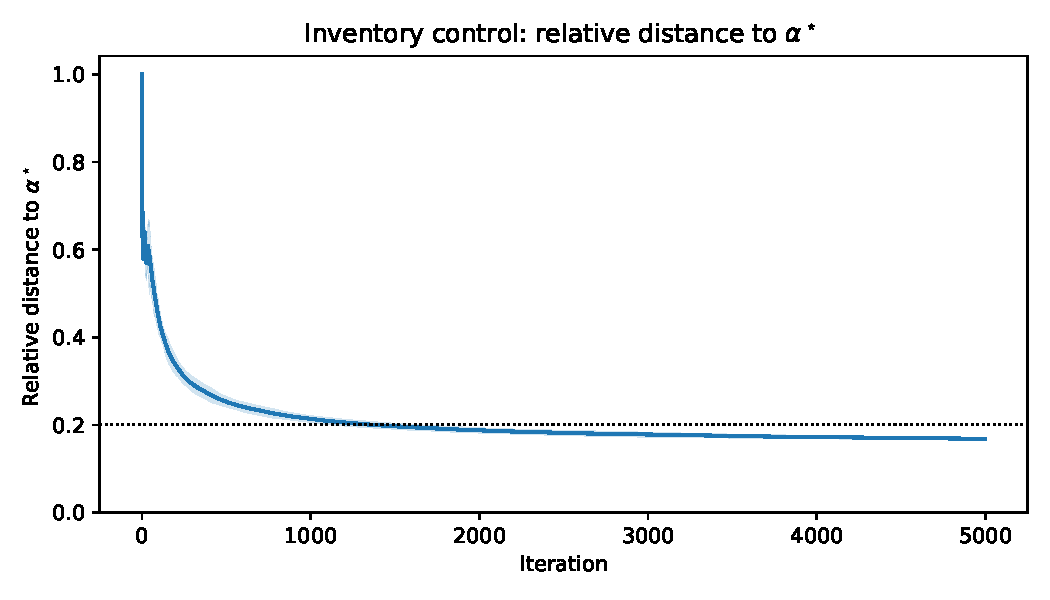
\includegraphics[width=0.75\textwidth]{../code/examples/optimal_control/inventory/sipm_inventory_gap_v3.pdf}
\caption{Inventory control: relative distance $\|\bar\alpha_k-\alpha^\star\|/\|\alpha^\star\|$
over iterations. The shaded region shows $\pm 3$ standard deviations,
and the dotted horizontal line indicates the level $0.2$.}
\label{fig:inventory-gap}
\end{figure}

To test the performance of our algorithm, we determie the ground-truth solution
with CVX \cite{diamond2016cvxpy}. Note that strong convexity of the objective,
along with the fact that we sample a finite amount of scenarios for the affine
constraints,
guarantee the existence of a unique minimizer
$\alpha^\star$ (see \cref{prop:strongly-convex-implies-lower-level-sets}).
We repeat the experiment over $10$ independent runs on the full dataset
and report the mean and standard deviation of the averaged iterates
$(\bar\alpha_k)_{k\in\mathbb{N}}$.
\Cref{fig:inventory-gap} shows the relative distance
$\|\bar\alpha_k-\alpha^\star\| / \|\alpha^\star\|$,
where $\alpha^\star$ denotes the unique empirical CVX minimiser,
together with $\pm 3$ standard deviation bands and a dotted reference
line at level $0.2$.
After $5000$ iterations, the final relative distance is
$1.68\times10^{-1} \pm 1.1\times10^{-3}$.
